\chapter{Experiments and Results}
\par To verify the functionality of CopeOpi vectors, we make comparisons with several commonly-used features for text classificaiton, and examine these features on different types of machine learning algorithms to solve text classification problems, including sentiment analysis and topic categorization, in both English and Chinese.
\section{Flowchart and Settings}
\par Figure~\ref{fig:flowchart} shows the flowchart of our experiments, detailed settings are described in the following sections.
\begin{figure}[h]
	\centering
	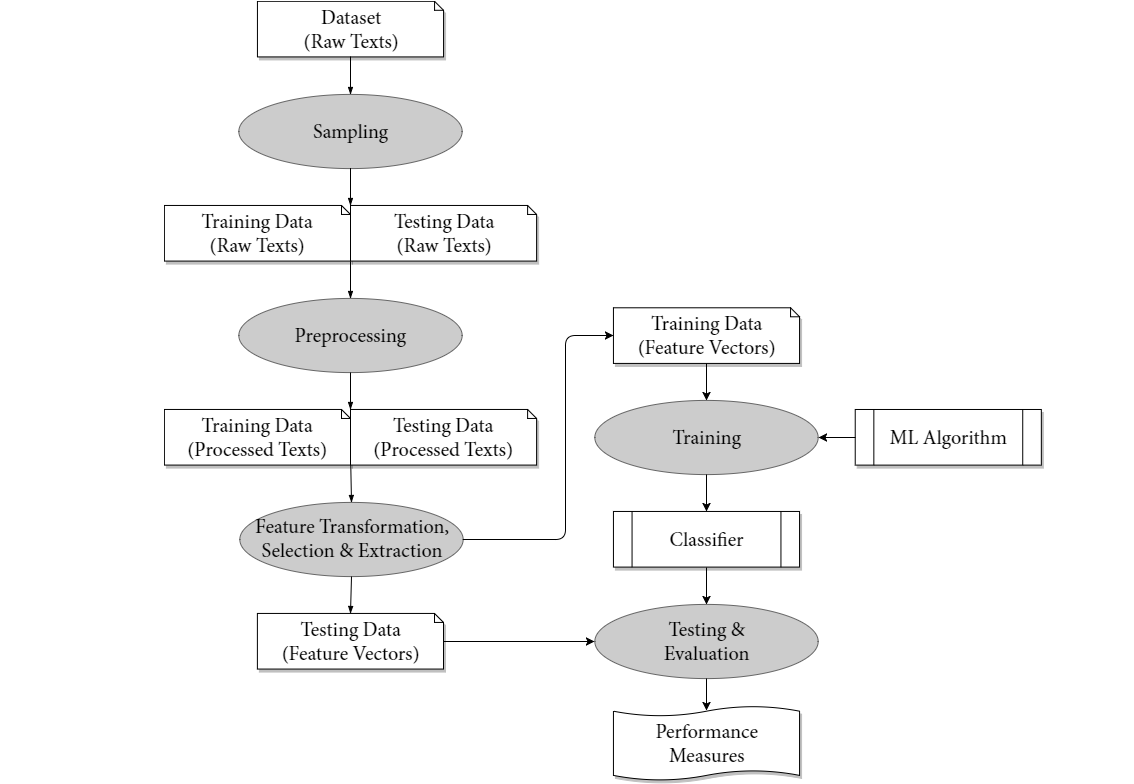
\includegraphics[scale=0.42]{chapters/ch4/figure/flowchart.png}
	\caption{The flowchart of experiments}
	\label{fig:flowchart}
\end{figure}
\par Table~\ref{tab:flow_opensrc} lists the open sources used in our experiments. They provide high quality implementation and ensure the reliability of experiment results.
\begin{table}[h]
\footnotesize
\centering
\caption{The open sources used in experiments}
\label{tab:flow_opensrc}
\begin{tabular}{|l|l|c|}
	\hline
	\multicolumn{1}{|c|}{Open Source}                                            & \multicolumn{1}{c|}{Functions}     & Reference                   \\ \hline
	\texttt{scikit-learn}\tablefootnote{http://scikit-learn.org}                 & Machine learning toolbox           & \cite{sklearn}              \\ \hline
	\texttt{gensim}\tablefootnote{http://radimrehurek.com/gensim}                & Nature language processing toolbox & \cite{gensim}               \\ \hline
	Stanford GloVe Project\tablefootnote{http://nlp.stanford.edu/projects/glove} & GloVe implementation                & \cite{pennington2014glove}  \\ \hline
	\texttt{jieba}\tablefootnote{http://github.com/fxsjy/jieba}                  & Chinese word segmenter             & \cite{jieba}                \\ \hline
\end{tabular}
\end{table}

\subsection{Sampling}
\par In most operational machine learning settings, once a classifier has been constructed, it is desirable to evaluate its performance. In this case, prior to classifier construction, the initial dataset is split into two parts\cite{sebastiani2002tc,ripley2007ml}:
\begin{itemize}
\item training set: a set of labeled instances used to construct a classifier, to fit the parameters of a machine learning algorithm.
	\begin{itemize}
	\item validation set: a set of labeled instances used to tune the hyperparameters of a machine learning algorithm.
	\end{itemize}
\item testing set: a set of labeled instances used to evaluate a classifier, to assess the performance of a fully-specified classifier.
\end{itemize}
~\newline
\partopic{Experiment Settings} are described in the sections of experiments.

\subsection{Preprocessing}
\par It is useful to apply some linguistic processing to raw texts before performing an analysis on them. Things to consider include:
\begin{itemize}
\item text cleaning: stripping unwanted tags, punctuation, numeric, etc.
\item tokenization: deciding what constitutes a unit and how to extract units.
\item normalization: converting superficially-different units to the same form.
\item stopword removal: removing frequent words which do not carry much meaning.
\end{itemize}
~\newline
\partopic{Experiment Settings} are described in Table~\ref{tab:flow_preproc}.
\par We unify the preprocessing for each language:
\begin{itemize}
\item for English corpora, we use \texttt{gensim.parsing.preprocessing.preprocess\_string} for text cleaning, tokenization, normalization and stopword removal.
\item for Chinese corpora, we use \texttt{jieba.cut} for tokenization; and strip characters outside the CJK Unified Ideographs\footnote{The Chinese, Japanese and Korean scripts share a common background, known as CJK characters.} UTF-8 block.
\end{itemize}
\begin{table}[h]
\footnotesize
\centering
\caption{Experiment settings of preprocessings}
\label{tab:flow_preproc}
\begin{tabular}{|c|m{0.205\textwidth}|c|m{0.13\textwidth}|c|}
	\hline
	Language & \multicolumn{1}{c|}{Text Cleaning}                                                            & Tokenization & \multicolumn{1}{c|}{Normalization} & Stopword Removal \\ \hline
	English  & Stripping tags,\newline punctuation,\newline multiple whitespaces,\newline numeric and shorts & Yes          & Lowercasing,\newline Stemming      & Yes              \\ \hline
	Chinese  & \multicolumn{1}{c|}{\texttt{[\textasciicircum \textbackslash u4E00-\textbackslash u9FFF]}}    & Yes          & \multicolumn{1}{c|}{No}            & No               \\ \hline
\end{tabular}
\end{table}

\subsection{Feature Transformation, Selection and Extraction}
Machine learning algorithms require a numerical representation of objects, so we have to transform documents as feature vectors before text classification. Due to the high-dimensional sparse property and the existence of irrelevant features, dimension reduction is especially important for texts\cite{aggarwal2012tc}:
\begin{itemize}
\item feature selection: picking a subset of features from the original feature set.
\item feature extraction: creating a new set of features from the original feature set.
\end{itemize}
~\newline
\partopic{Experiment Settings} are described in Table~\ref{tab:flow_features}.
\par We make comparisons with several commonly-used features for text classificaiton, including:
\begin{itemize}
\item term-document matrix models:
	\begin{itemize}
	\item bag-of-word (BOW)
	\item LSI\cite{deerwester1990lsi}-truncated BOW (BOW(LSI))
	\item term frequency-inverse document frequency (TF-IDF)
	\item LSI-truncated TF-IDF (TF-IDF(LSI))
	\end{itemize}
\item word-context matrix models:
	\begin{itemize}
	\item Word2vec\cite{mikolov2013word2vec}
	\item GloVe\cite{pennington2014glove}
	\end{itemize}
\end{itemize}
\begin{table}[h]
\footnotesize
\centering
\caption{Experiment settings of features}
\label{tab:flow_features}
\begin{tabular}{|l|m{0.495\textwidth}|m{0.09\textwidth}|c|}
	\hline
	\multicolumn{1}{|c|}{Feature} & \multicolumn{1}{c|}{Implementaion}                                                                            & \multicolumn{1}{c|}{Feature Selection} & Normalized \\ \hline
	CopeOpi                       & Our implementaion                                                                                             & \texttt{min\_count=5}                  & Yes        \\ \hline
	BOW                           & \texttt{sklearn.feature\_extraction.text.CountVectorizer}                                                     & \texttt{min\_df=0.001}                 & No         \\ \hline
	BOW(LSI)                      & \texttt{sklearn.feature\_extraction.text.CountVectorizer}\newline \texttt{sklearn.decomposition.TruncatedSVD} & \texttt{min\_df=0.001}                 & Yes        \\ \hline
	TF-IDF                        & \texttt{sklearn.feature\_extraction.text.TfidfVectorizer}                                                     & \texttt{min\_df=0.001}                 & Yes        \\ \hline
	TF-IDF(LSI)                   & \texttt{sklearn.feature\_extraction.text.TfidfVectorizer}\newline \texttt{sklearn.decomposition.TruncatedSVD} & \texttt{min\_df=0.001}                 & Yes        \\ \hline
	Word2vec                      & \texttt{gensim.models.word2vec}                                                                               & \texttt{min\_count=5}                  & Yes        \\ \hline
	GloVe                         & Stanford GloVe Project                                                                                        & \texttt{min\_count=5}                  & Yes        \\ \hline
\end{tabular}
\end{table}

\subsection{Training}
Since documents may be represented as feature vectors, it is possible to use most machine learning algorithms for text classification, as we discussed in section~\ref{sec:ml}.
~\newline
~\newline
\partopic{Experiment Settings} are described in Table~\ref{tab:flow_mlalgos}.
\par We examine the mentioned features on different types of machine learning algorithms, including:
\begin{itemize}
\item k-Nearest neighbor classifiers (kNN)
\item naive Bayes classifiers (NB)
\item logistic regression classifiers (LR)
\item support vector machine classifiers (SVM)
\item neural network classifiers (NN)
\end{itemize}
\begin{table}[h]
\footnotesize
\centering
\caption{Experiment settings of machine learning algorithms}
\label{tab:flow_mlalgos}
\begin{tabular}{|l|m{0.565\textwidth}|}
	\hline
	\multicolumn{1}{|c|}{Machine Learining Algorithm} & \multicolumn{1}{c|}{Implementaion}                                                                                                                           \\ \hline
	k-Nearest Neighbor (kNN)                          & \texttt{sklearn.neighbors.KNeighborsClassifier(n\_neighbors=40)}                                                                                             \\ \hline
	Naive Bayes (NB)                                  & \parbox{0.385\textwidth}{\texttt{sklearn.naive\_bayes.MultinomialNB}} for BOW, TF-IDF\newline \parbox{0.385\textwidth}{\texttt{sklearn.naive\_bayes.GaussianNB}} for the others\\ \hline
	Logistic Regression (LR)                          & \texttt{sklearn.linear\_model.LogisticRegression}                                                                                                            \\ \hline
	Support Vector Machine (SVM)                      & \texttt{sklearn.svm.LinearSVC}                                                                                                                               \\ \hline
	Neural Network (NN)                               & \texttt{sklearn.neural\_network.MLPClassifier}                                                                                                               \\ \hline
\end{tabular}
\end{table}

\subsection{Testing and Evaluation}
Table~\ref{tab:flow_prf1} is the contingency table of binary classification. Performance of a binary classifier is usually measured in terms of precision, recall and \fscore{}\cite{sebastiani2002tc}, which are defined as follows:
\begin{itemize}
\item precision: the fraction of predicted-true that are real-true.
\item recall: the fraction of the real-true that are predicted-true.
\item \fscore{}: the harmonic mean of precision and recall.
\begin{equation*}
\begin{gathered}
	\precision_c = \dfrac{{TP}_c}{{TP}_c+{FP}_c}
\\[\eqlineskip]
	\recall_c = \dfrac{{TP}_c}{{TP}_c+{FN}_c}
\\[\eqlineskip]
	{F_1}_c = \dfrac{2 \times \precision_c \times \recall_c}{\precision_c + \recall_c}
\end{gathered}
\end{equation*}
\end{itemize}
\vspace{-\intextsep}
\begin{table}[h]
\footnotesize
\centering
\caption{The contingency table of binary classification}
\label{tab:flow_prf1}
\begin{tabular}{lc|c|c|}
	\hline
	\multicolumn{2}{|l|}{\multirow{2}{*}{}}                             & \multicolumn{2}{c|}{Real}                                                                                           \\ \cline{3-4} 
	\multicolumn{2}{|l|}{}                                              & $\mathtt{True}$     & $\mathtt{False}$    \\ \hline
	\multicolumn{1}{|c|}{\multirow{2}{*}{Predicted}} & $\mathtt{True}$  & True positive (TP)  & False positive (FP) \\ \cline{2-4} 
	\multicolumn{1}{|c|}{}                           & $\mathtt{False}$ & False negative (FN) & True negative (TN)  \\ \hline
\end{tabular}
\end{table}
~\newline
\partopic{Experiment Settings}
\par As for multiclass classification, we use \fscore{} as measure for each class, and take average of them as a macro \fscore{}.
\begin{equation*}
	\mathrm{macro}\text{-}F_1 = \dfrac{1}{|\mathbb{C}|} \sum_{c \in \mathbb{C}} {F_1}_c
\end{equation*}


\section{Experiments: Sentiment Analysis}
We use SA($lang$)($n$) as the abbreviation standing for sentiment analysis experiment $n$ of language $lang$, where EN represents English and ZH represents Chinese.
\subsection{Datasets}
We use Yelp Dataset\footnote{The version we use is Yelp Dataset Challenge round 9.}\cite{Yelp} as the English corpus and MioChnCorp\cite{MioChnCorp} as the Chinese corpus.
Both are user-assigned five-star integral rating sentiment annotated, ranged from 5 as positive to 1 as negative. 
Table~\ref{tab:sa_data} is the descriptions about these datasets.
~\newline
~\newline
\partopic{Experiment Datasets} are summarized in Table~\ref{tab:sa_dataexp}.
\par We randomly select 15000 instances from the original dataset for each experiment, and split into a training set and a testing set in ratio 0.5:0.5.
\begin{itemize}
\item SA(EN|ZH)(A): 2 classes are positive and negative.
\item SA(EN|ZH)(B): 3 classes are positive, negative and neutral.
\item SA(EN|ZH)(C): 5 classes are 1-star, 2-star, 3-star, 4-star and 5-star.
\end{itemize}
\begin{table}[]
\centering
\caption{Sentiment analysis datasets}
\label{tab:sa_data}
\begin{tabular}{|l|c|m{0.3\textwidth}|c|c|}
\hline
Name      & Language & \multicolumn{1}{c|}{Description}
              & \multicolumn{1}{c|}{Source} \\ \hline
Yelp Dataset\cite{Yelp9} & English           & Customer reviews about local business such as restaurants, hair stylists, mechanics, etc.
                                  & Yelp \\ \hline
MioChnCorp\cite{MioChnCorp}   & Chinese           & Customer reviews about hotels.
                          & Dianping \\ \hline
\end{tabular}
\end{table}
\vspace{-\intextsep}
\begin{table}[]
\centering
\caption{Sentiment analysis experiments datasets}
\begin{tabular}{|c|c|c|c|c|c|}
\hline
     & Rating-1      & Rating-2      & Rating-3 & Rating-4      & Rating-5      \\ \hline
SA(A)(2) & \multicolumn{2}{c|}{Negative} &          & \multicolumn{2}{c|}{Positive} \\ \hline
SA(B)(3) & Negative      &               & Neutral  &               & Positive      \\ \hline
SA(C)(5) & Rating-1      & Rating-2      & Rating-3 & Rating-4      & Rating-5      \\ \hline
\end{tabular}
\end{table}

\subsection{Results and Observations}
\par We use macro \fscore{}s as the measure of effectiveness and training CPU time as the measure of efficiency. Results\footnote{The values of \fscore{}s are the larger the better, while the values of training CPU time are the smaller the better. In the table of results, color green represents a better result while color red represents a worse result; three bold values are the top three results of each classifier.} are shown in Table~\ref{tab:sa_en_a} to Table~\ref{tab:sa_zh_c}.
\par Here we brief our observations about the results of sentiment analysis experiments:
\begin{enumerate}
\item In SA(EN)(A) and SA(ZH)(A),
which are binary text classification problems, the CopeOpi here are augmented CopeOpi scores.
Compare the best macro \fscore{} of CopeOpi and the best macro \fscore{} of each experiment, we lose by
4.57\% in SA(EN)(A) and 2.08\% in SA(ZH)(A).
This shows that the computation scheme of augmented CopeOpi scores is feasible in both English and Chinese binary text classification.
\item In SA(ZH)(A),
which is a binary Chinese sentiment analysis problem, we compare with the CopeOpi scores recorded in ANTUSD\cite{wang2006antusd}, which are original CopeOpi scores.
The augmented CopeOpi scores outperform the CopeOpi scores recorded in ANTUSD by more than 10\% for each classifier.
This shows that augmented CopeOpi scores function normally without manually filtering irrelevant words and are more applicable to the dataset.
\item In SA(EN)(B), SA(EN)(C), SA(ZH)(B) and SA(ZH)(C),
which are multiclass text classification problems, the CopeOpi here are CopeOpi vectors constructed by one-versus-rest, one-versus-one and both strategies.
Compare the best macro \fscore{} of CopeOpi and the best macro \fscore{} of each experiment, we lose by
2.10\% in SA(EN)(B), 2.58\% in SA(EN)(C), 0.42\% in SA(ZH)(B) and 1.30\% in SA(ZH)(C).
This shows that the computation scheme of CopeOpi vectors is feasible in both English and Chinese multiclass text classification.
\item
$\frac{4}{10}$ of the macro \fscore{}s of CopeOpi scores in SA(EN|ZH)(A) are better than the average macro \fscore{} of each classifier of each experiment,
$\frac{18}{20}$ of the best macro \fscore{}s of CopeOpi vectors in SA(EN|ZH)(B|C) are better than the average macro \fscore{} of each classifier of each experiment.
This shows that CopeOpi vectors in muticlass classification are more effective than augmented CopeOpi scores in binary classification.
\end{enumerate}

\begin{table}[H]
\caption{Results of SA(EN)(A)}
\label{tab:sa_en_a}
\centering
\begin{subtable}{\textwidth}
	\centering
	\caption{Macro \fscore{}}
	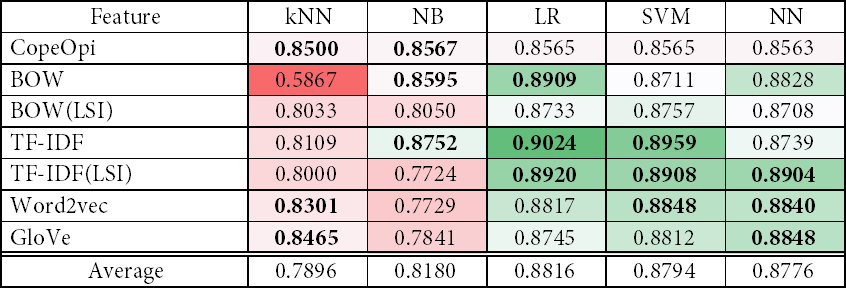
\includegraphics[width=\resultfigwidth]{chapters/ch4/table/sa/SA(EN)(A).png}
\end{subtable}
\\[\tblskip]
\begin{subtable}{\textwidth}
	\centering
	\caption{Training CPU Time}
	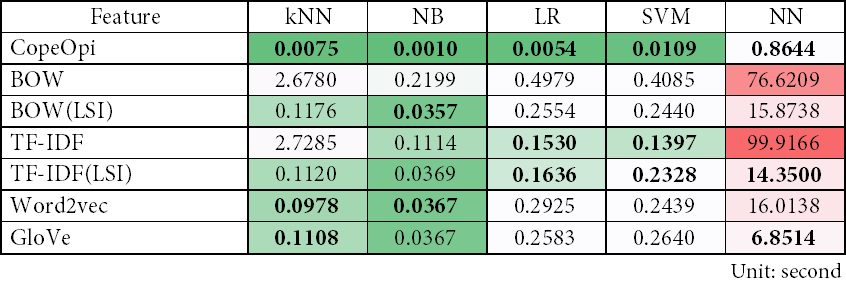
\includegraphics[width=\resultfigwidth]{chapters/ch4/table/sa/SA(EN)(A)T.png}
\end{subtable}
\end{table}
\vspace{-1.75\intextsep}
\begin{table}[H]
\caption{Results of SA(EN)(B)}
\label{tab:sa_en_b}
\centering
\begin{subtable}{\textwidth}
	\centering
	\caption{Macro \fscore{}}
	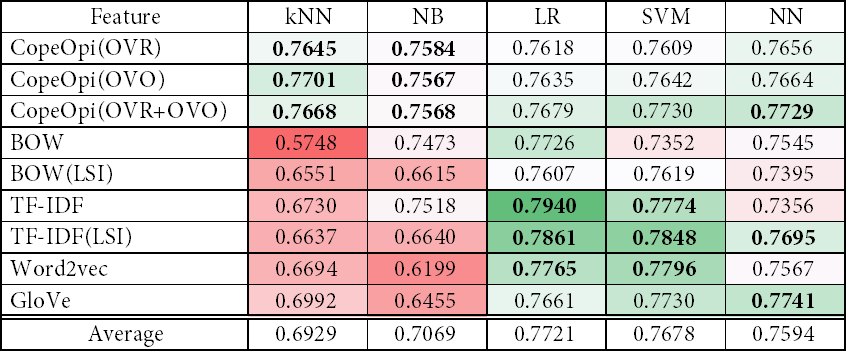
\includegraphics[width=\resultfigwidth]{chapters/ch4/table/sa/SA(EN)(B).png}
\end{subtable}
\\[\tblskip]
\begin{subtable}{\textwidth}
	\centering
	\caption{Training CPU Time}
	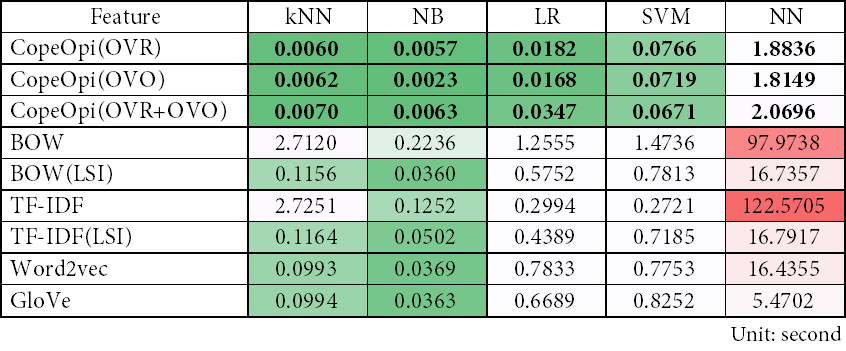
\includegraphics[width=\resultfigwidth]{chapters/ch4/table/sa/SA(EN)(B)T.png}
\end{subtable}
\end{table}
\begin{table}[H]
\caption{Results of SA(EN)(C)}
\label{tab:sa_en_c}
\centering
\begin{subtable}{\textwidth}
	\centering
	\caption{Macro \fscore{}}
	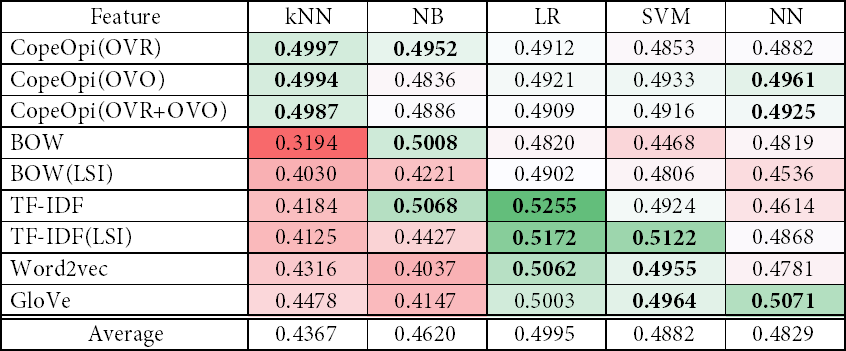
\includegraphics[width=\resultfigwidth]{chapters/ch4/table/sa/SA(EN)(C).png}
\end{subtable}
\\[\tblskip]
\begin{subtable}{\textwidth}
	\centering
	\caption{Training CPU Time}
	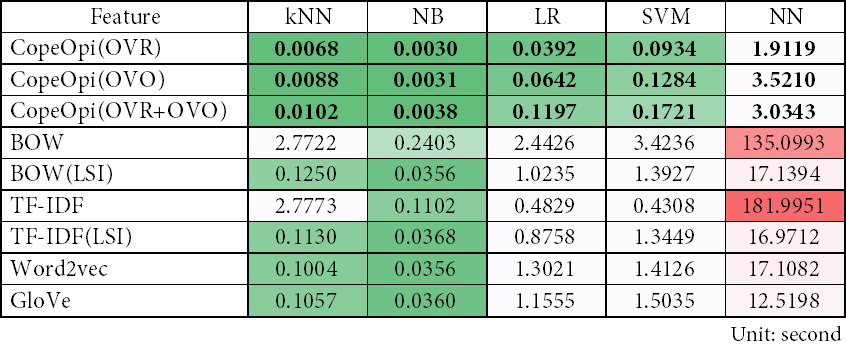
\includegraphics[width=\resultfigwidth]{chapters/ch4/table/sa/SA(EN)(C)T.png}
\end{subtable}
\end{table}
\vspace{-1.75\intextsep}
%\begin{table}
\caption{Results of SA(ZH)(A)}
\label{tab:sa_zh_a}
\centering
\begin{subtable}{\textwidth}
	\centering
	\caption{F1-scores of SA(ZH)(A)}
	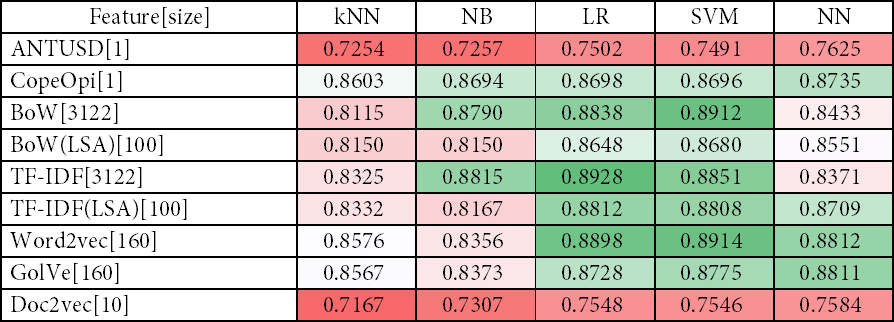
\includegraphics[width=0.8\textwidth]{./figure/02A1.png}
\end{subtable}\\[1em]
\begin{subtable}{\textwidth}
	\centering
	\caption{Training CPU Time of SA(ZH)(A)}
	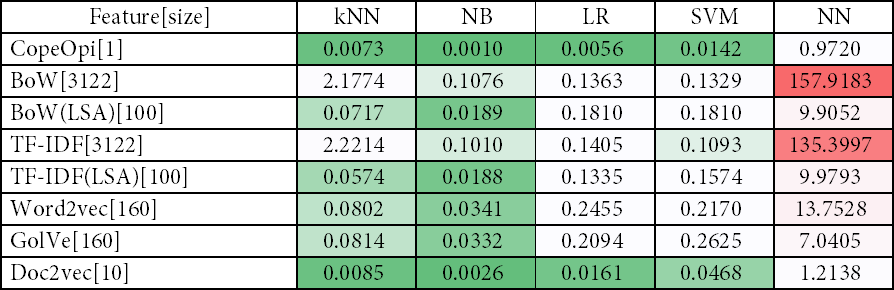
\includegraphics[width=0.8\textwidth]{./figure/02A1t.png}
\end{subtable}
%\end{table}
\begin{table}[H]
\caption{Results of SA(ZH)(B)}
\label{tab:sa_zh_b}
\centering
\begin{subtable}{\textwidth}
	\centering
	\caption{Macro \fscore{}}
	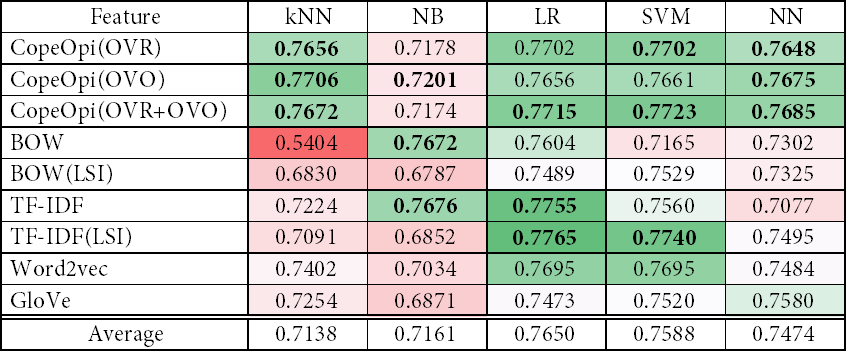
\includegraphics[width=\resultfigwidth]{chapters/ch4/table/sa/SA(ZH)(B).png}
\end{subtable}
\\[\tblskip]
\begin{subtable}{\textwidth}
	\centering
	\caption{Training CPU Time}
	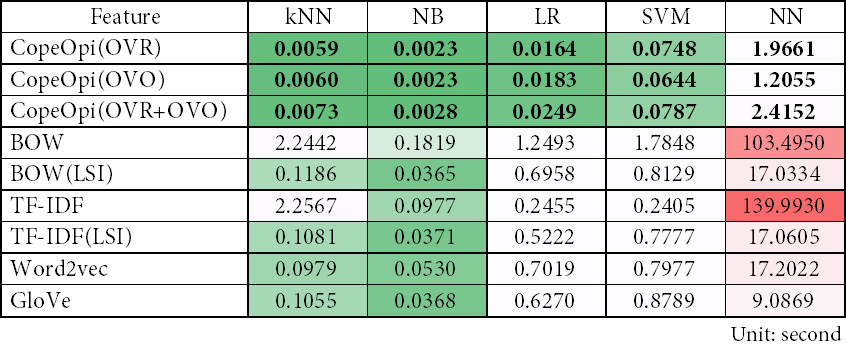
\includegraphics[width=\resultfigwidth]{chapters/ch4/table/sa/SA(ZH)(B)T.png}
\end{subtable}
\end{table}
\vspace{-1.75\intextsep}
\begin{table}[H]
\caption{Results of SA(ZH)(C)}
\label{tab:sa_zh_c}
\centering
\begin{subtable}{\textwidth}
	\centering
	\caption{Macro \fscore{}}
	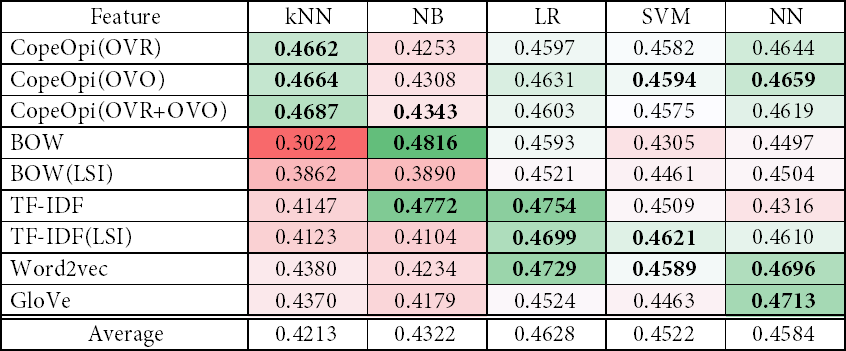
\includegraphics[width=\resultfigwidth]{chapters/ch4/table/sa/SA(ZH)(C).png}
\end{subtable}
\\[\tblskip]
\begin{subtable}{\textwidth}
	\centering
	\caption{Training CPU Time}
	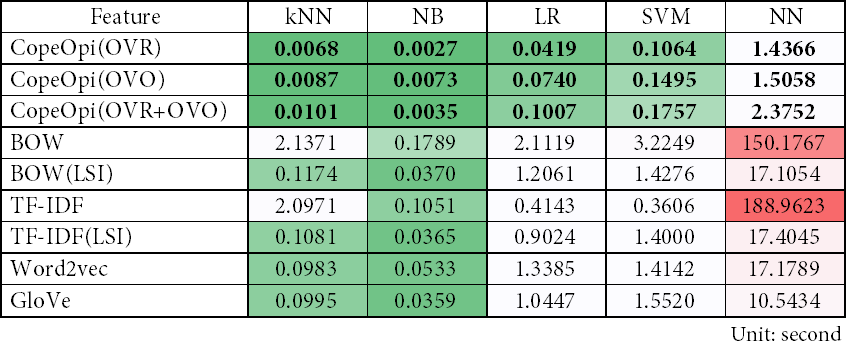
\includegraphics[width=\resultfigwidth]{chapters/ch4/table/sa/SA(ZH)(C)T.png}
\end{subtable}
\end{table}


\section{Experiments: Topic Categorization}
We use TC($lang$)($n$) as the abbreviation standing for topic categorization experiment $n$ of language $lang$, where EN represents English and ZH represents Chinese.
\subsection{Datasets}
We use 20 Newsgroups\cite{20news} as the English corpus and Fudan University TC Corpus\cite{fudan} as the Chinese corpus.
Both contains 20 categories and training-and-testing splits.
Table~\ref{tab:tc_data} is the descriptions about these datasets.
~\newline
~\newline
\partopic{Experiment Datasets} are summarized in Table~\ref{tab:tc_dataexp}.
\par We subset categories from the original dataset for each experiment, and use their default training-and-testing splits.
\begin{itemize}
\item TC(EN):
	\begin{itemize}
	\item TC(EN)(A): 20 classes are all categories of the original dataset.
	\item TC(EN)(B): 7 classes are the first hierarchy categories.
	\item TC(EN)(C): 5 classes are categories within the first hierarchy comp.
	\item TC(EN)(D): 4 classes are categories within the first hierarchy talk.
	\end{itemize}
\item TC(ZH):
	\begin{itemize}
	\item TC(ZH)(A): 20 classes are all categories of the original dataset.
	\item TC(ZH)(B): 9 classes are categories with more than a hundred instances.
	\item TC(ZH)(C): 11 classes are categories with less than a hundred instances.
	\end{itemize}
\end{itemize}
\begin{table}[h]
\footnotesize
\centering
\caption{Topic categorization datasets}
\label{tab:tc_data}
\begin{tabular}{|l|c|c|c|c|}
	\hline
	\multicolumn{1}{|c|}{Dataset} & Language & \# of Classes & Balanced & Train:Test \\ \hline
	20 Newsgroup                  & English  & 20            & Yes      & 0.6:0.4    \\ \hline
	Fudan University TC Corpus    & Chinese  & 20            & No       & 0.5:0.5    \\ \hline
\end{tabular}
\end{table}
\begin{table}[h]
\footnotesize
\centering
\begin{minipage}{\textwidth}
\caption{Topic categorization experiments datasets}
\label{tab:tc_dataexp}
\begin{subtable}{0.58\textwidth}
\centering
\caption{Sampling of TC(EN)}
\scalebox{0.72}{
\begin{tabular}{|l|c|c|c|c|}
	\hline
	\multicolumn{1}{|c|}{Classes} & (A)        & (B)                        & (C)       & (D)       \\ \hline
	alt.atheism                   & 480:319    & 480:319                    &           &           \\ \hline
	comp.graphics                 & 584:389    & \multirow{5}{*}{2936:1955} & 584:389   &           \\ \cline{1-2} \cline{4-5} 
	comp.os.ms-windows.misc       & 591:394    &                            & 591:394   &           \\ \cline{1-2} \cline{4-5} 
	comp.sys.ibm.pc.hardware      & 590:392    &                            & 590:392   &           \\ \cline{1-2} \cline{4-5} 
	comp.sys.mac.hardware         & 578:385    &                            & 578:385   &           \\ \cline{1-2} \cline{4-5} 
	comp.windows.x                & 593:395    &                            & 593:395   &           \\ \hline
	misc.forsale                  & 585:390    & 585:390                    &           &           \\ \hline
	rec.autos                     & 594:396    & \multirow{4}{*}{2389:1590} &           &           \\ \cline{1-2} \cline{4-5}
	rec.motorcycles               & 598:398    &                            &           &           \\ \cline{1-2} \cline{4-5} 
	rec.sport.baseball            & 597:397    &                            &           &           \\ \cline{1-2} \cline{4-5} 
	rec.sport.hockey              & 600:399    &                            &           &           \\ \hline
	sci.crypt                     & 595:396    & \multirow{4}{*}{2373:1579} &           &           \\ \cline{1-2} \cline{4-5} 
	sci.electronics               & 591:393    &                            &           &           \\ \cline{1-2} \cline{4-5} 
	sci.med                       & 594:396    &                            &           &           \\ \cline{1-2} \cline{4-5} 
	sci.space                     & 593:394    &                            &           &           \\ \hline
	soc.religion.christian        & 599:398    & 599:398                    &           &           \\ \hline
	talk.politics.guns            & 546:364    & \multirow{4}{*}{1952:1301} &           & 546:364   \\ \cline{1-2} \cline{4-5}
	talk.politics.mideast         & 564:376    &                            &           & 564:376   \\ \cline{1-2} \cline{4-5}
	talk.politics.misc            & 465:310    &                            &           & 465:310   \\ \cline{1-2} \cline{4-5}
	talk.religion.misc            & 377:251    &                            &           & 377:251   \\ \hline
	\multicolumn{1}{|c|}{Total}   & 11314:7532 & 11314:7532                 & 2936:1955 & 1952:1301 \\ \hline
\end{tabular}}
\end{subtable}
\begin{subtable}{0.42\textwidth}
\centering
\caption{Sampling of TC(ZH)}
\scalebox{0.72}{
\begin{tabular}{|l|c|c|c|}
	\hline
	\multicolumn{1}{|c|}{Classes} & (A)       & (B)       & (C)     \\ \hline
	Art                           & 740:742   & 740:742   &         \\ \hline
	Literature                    & 33:34     &           & 33:34   \\ \cline{1-2} \cline{3-4}
	Education                     & 59:61     &           & 59:61   \\ \cline{1-2} \cline{3-4}
	Philosophy                    & 44:45     &           & 44:45   \\ \cline{1-2} \cline{3-4}
	History                       & 466:468   & 466:468   &         \\ \cline{1-2} \cline{3-4}
	Space                         & 640:642   & 640:642   &         \\ \hline
	Energy                        & 32:33     &           & 32:33   \\ \hline
	Electronics                   & 27:28     &           & 27:28   \\ \cline{1-2} \cline{3-4}
	Communication                 & 25:27     &           & 25:27   \\ \cline{1-2} \cline{3-4}
	Computer                      & 1357:1358 & 1357:1358 &         \\ \cline{1-2} \cline{3-4}
	Mine                          & 33:34     &           & 33:34   \\ \hline
	Transport                     & 57:59     &           & 57:59   \\ \cline{1-2} \cline{3-4}
	Environment                   & 1217:1218 & 1217:1218 &         \\ \cline{1-2} \cline{3-4}
	Agriculture                   & 1021:1022 & 1021:1022 &         \\ \cline{1-2} \cline{3-4}
	Economy                       & 1600:1601 & 1600:1601 &         \\ \hline
	Law                           & 51:52     &           & 51:52   \\ \hline
	Medical                       & 51:53     &           & 51:53   \\ \cline{1-2} \cline{3-4}
	Military                      & 74:76     &           & 74:76   \\ \cline{1-2} \cline{3-4}
	Politics                      & 1024:1026 & 1024:1026 &         \\ \cline{1-2} \cline{3-4}
	Sports                        & 1253:1254 & 1253:1254 &         \\ \hline
	\multicolumn{1}{|c|}{Total}   & 9804:9833 & 9318:9331 & 486:502 \\ \hline
\end{tabular}}
\end{subtable}
\end{minipage}
\end{table}

\subsection{Results and Observations}
\par We use macro \fscore{}s as the measure of effectiveness and training CPU time as the measure of efficiency. Results\footnote{The values of \fscore{}s are the larger the better, while the values of training CPU time are the smaller the better. In the table of results, color green represents a better result while color red represents a worse result; three bold values are the top three results of each classifier.} are shown in Table~\ref{tab:tc_en_a} to Table~\ref{tab:tc_zh_c}.
\par Here we brief our observations about the results of topic categorization experiments:
\begin{enumerate}
\item
	\begin{enumerate}[label=(\roman*)]
	\item In TC(EN)(A) and TC(ZH)(A),
	both corpora contain 20 categories.
	Compare the best macro \fscore{} of CopeOpi and the best macro \fscore{} of each experiment, we lose by
	0.87\% in TC(EN)(A) but 14.01\% in TC(ZH)(A).
	CopeOpi vectors function badly in one of them.
	Except languages, the biggest difference between their corpus is the balance.
	But we doubt if CopeOpi vectors can not function well in imbalanced corpora since the influence of imbalance should be smoothed by the normalization of their formulas.
	\item In TC(EN)(B) and TC(ZH)(A),
	both corpora are imbalanced.
	Compare the best macro \fscore{} of CopeOpi and the best macro \fscore{} of each experiment, we lose by
	1.03\% in TC(EN)(B) but 14.01\% in TC(ZH)(A).
	CopeOpi vectors function well in one of them.
	Except languages, the biggest difference between their corpus is the size of the training set.
	We deduce that the reason why CopeOpi vectors function badly in TC(ZH)(A) is due to the lack of training instances, not imbalance.
	\end{enumerate}
\item In TC(ZH)(B) and TC(ZH)(C),
the former corpus contains categories with more than a hundred instances, the later corpus contains categories with less than a hundred instances.
Compare the best macro \fscore{} of CopeOpi and the best macro \fscore{} of each experiment, we lose by
3.02\% in TC(ZH)(B) but 8.95\% in TC(ZH)(C).
This confirms the deduction that CopeOpi vectors can not function well if there are no sufficient training instances. 
\item In TC(EN)(C) and TC(EN)(D),
both corpora contain categories with similar topics.
Compare the best macro \fscore{} of CopeOpi and the best macro \fscore{} of each experiment, we lose by
2.33\% in TC(EN)(C) and 0.51\% in TC(EN)(D).
This shows that CopeOpi vectors can function well even though categories are similar.
\end{enumerate}
%\begin{table}
\caption{Results of TC(EN)(A)}
\label{tab:tc_en_a}
\centering
\begin{subtable}{\textwidth}
	\centering
	\caption{F1-scores of TC(EN)(A)}
	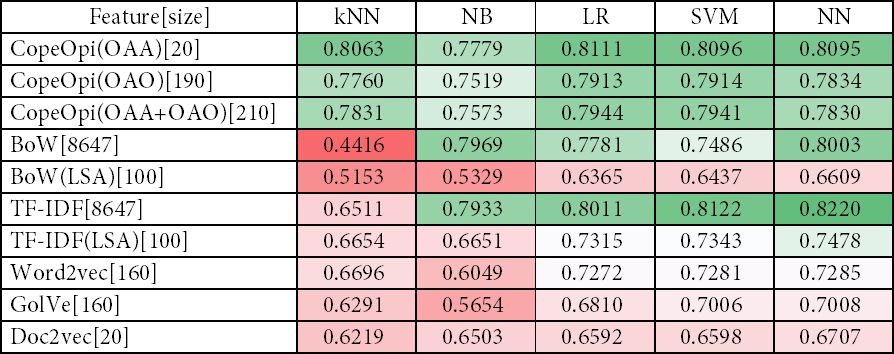
\includegraphics[width=0.8\textwidth]{./figure/01B1.png}
\end{subtable}\\[1em]
\begin{subtable}{\textwidth}
	\centering
	\caption{Training CPU Time of TC(EN)(A)}
	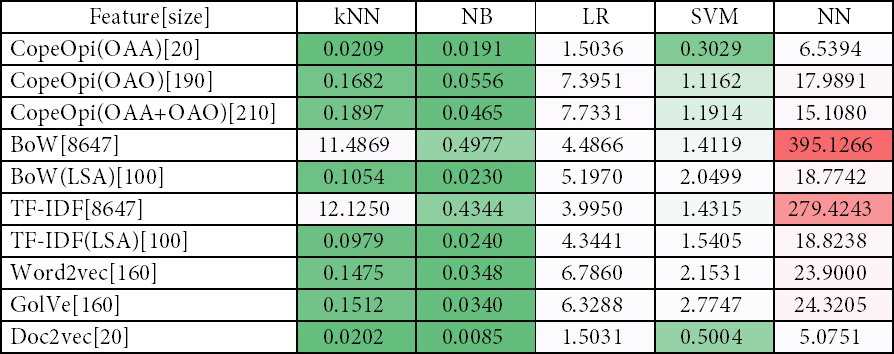
\includegraphics[width=0.8\textwidth]{./figure/01B1t.png}
\end{subtable}
%\end{table}
%\begin{table}
\caption{Results of TC(EN)(B)}
\label{tab:tc_en_b}
\centering
\begin{subtable}{\textwidth}
	\centering
	\caption{F1-scores of TC(EN)(B)}
	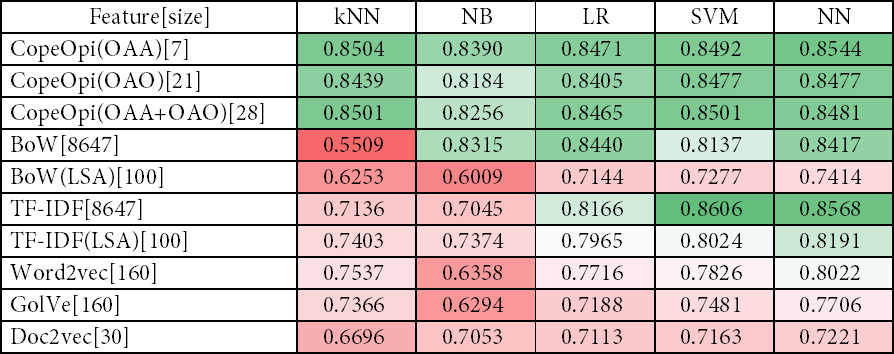
\includegraphics[width=0.8\textwidth]{./figure/01B2.png}
\end{subtable}\\[1em]
\begin{subtable}{\textwidth}
	\centering
	\caption{Training CPU Time of TC(EN)(B)}
	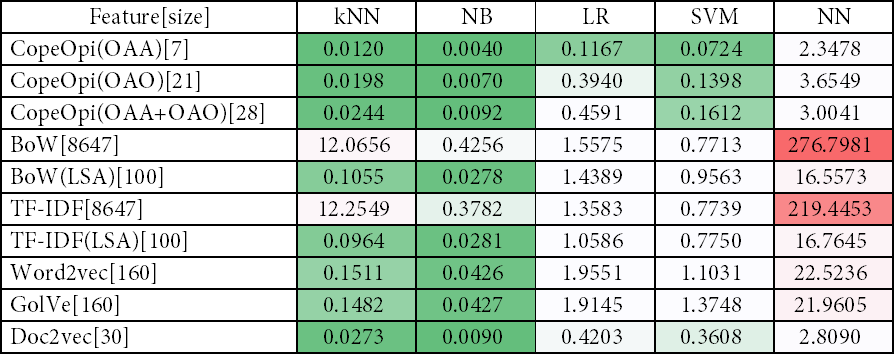
\includegraphics[width=0.8\textwidth]{./figure/01B2t.png}
\end{subtable}
%\end{table}
\vspace{-1.75\intextsep}
%\begin{table}
\caption{Results of TC(EN)(C)}
\label{tab:tc_en_c}
\centering
\begin{subtable}{\textwidth}
	\centering
	\caption{F1-scores of TC(EN)(C)}
	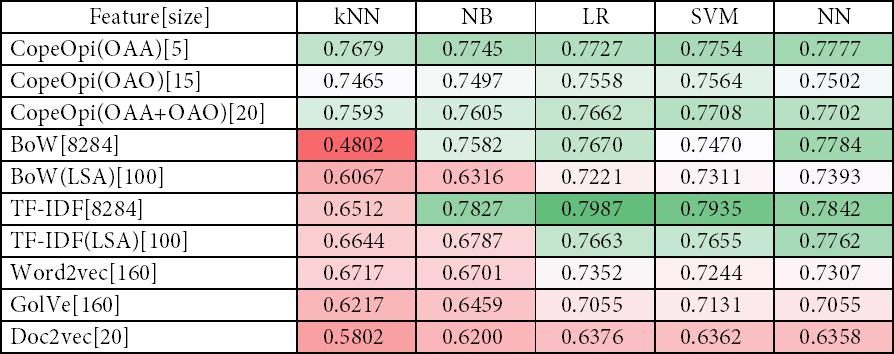
\includegraphics[width=0.8\textwidth]{./figure/01B3.png}
\end{subtable}\\[1em]
\begin{subtable}{\textwidth}
	\centering
	\caption{Training CPU Time of TC(EN)(C)}
	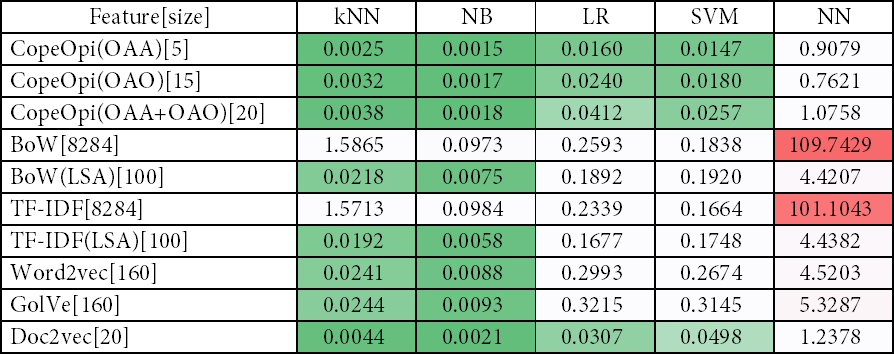
\includegraphics[width=0.8\textwidth]{./figure/01B3t.png}
\end{subtable}
%\end{table}
\begin{table}[H]
\caption{Results of TC(EN)(D)}
\label{tab:tc_en_d}
\centering
\begin{subtable}{\textwidth}
	\centering
	\caption{Macro \fscore{}}
	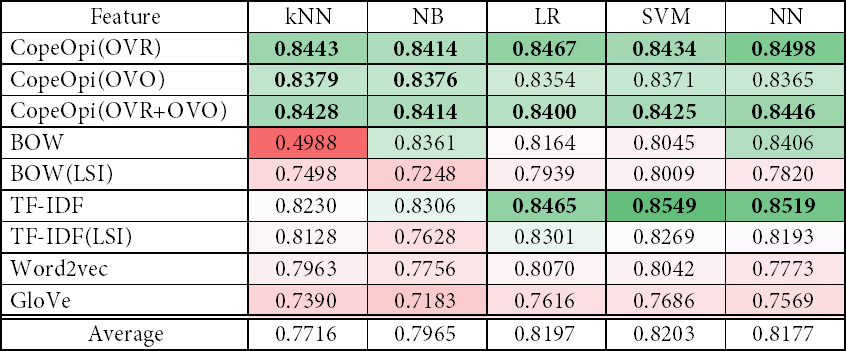
\includegraphics[width=\resultfigwidth]{chapters/ch4/table/tc/TC(EN)(D).png}
\end{subtable}
\\[\tblskip]
\begin{subtable}{\textwidth}
	\centering
	\caption{Training CPU Time}
	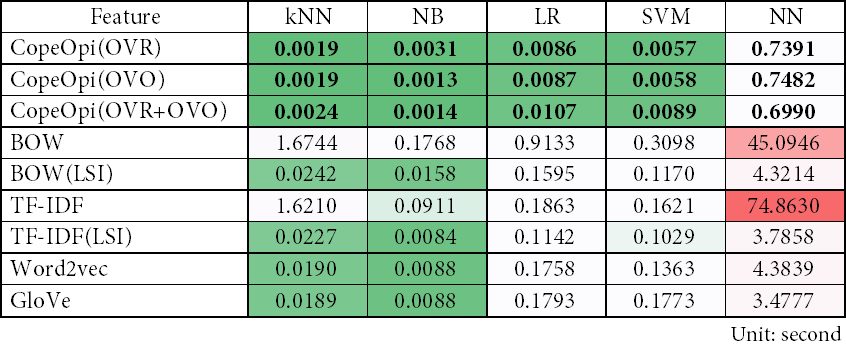
\includegraphics[width=\resultfigwidth]{chapters/ch4/table/tc/TC(EN)(D)T.png}
\end{subtable}
\end{table}
\vspace{-1.75\intextsep}
%\begin{table}
\caption{Results of TC(ZH)(A)}
\label{tab:tc_zh_a}
\centering
\begin{subtable}{\textwidth}
	\centering
	\caption{F1-scores of TC(ZH)(A)}
	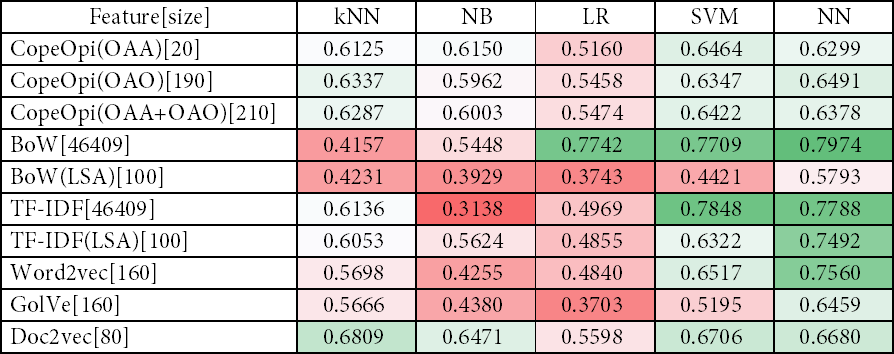
\includegraphics[width=0.8\textwidth]{./figure/02B1.png}
\end{subtable}\\[1em]
\begin{subtable}{\textwidth}
	\centering
	\caption{Training CPU Time of TC(ZH)(A)}
	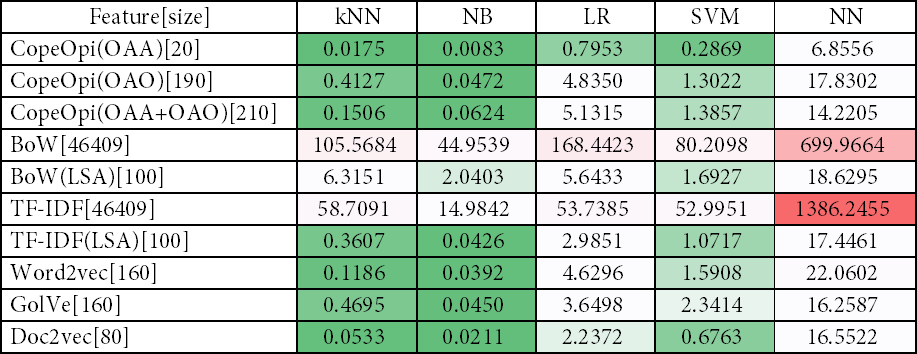
\includegraphics[width=0.8\textwidth]{./figure/02B1t.png}
\end{subtable}
%\end{table}
\begin{table}[H]
\caption{Results of TC(ZH)(B)}
\label{tab:tc_zh_b}
\centering
\begin{subtable}{\textwidth}
	\centering
	\caption{Macro \fscore{}}
	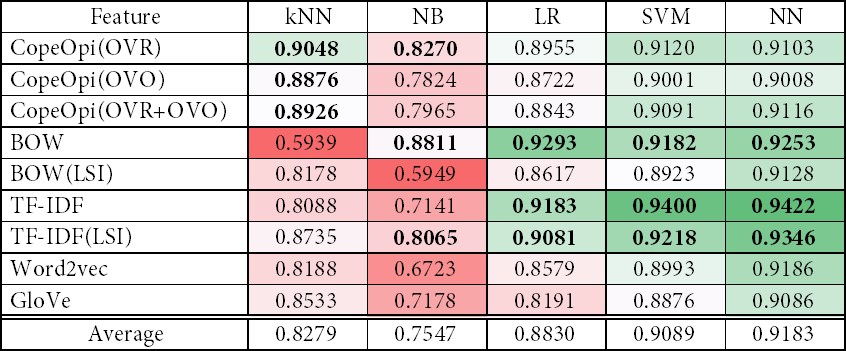
\includegraphics[width=\resultfigwidth]{chapters/ch4/table/tc/TC(ZH)(B).png}
\end{subtable}
\\[\tblskip]
\begin{subtable}{\textwidth}
	\centering
	\caption{Training CPU Time}
	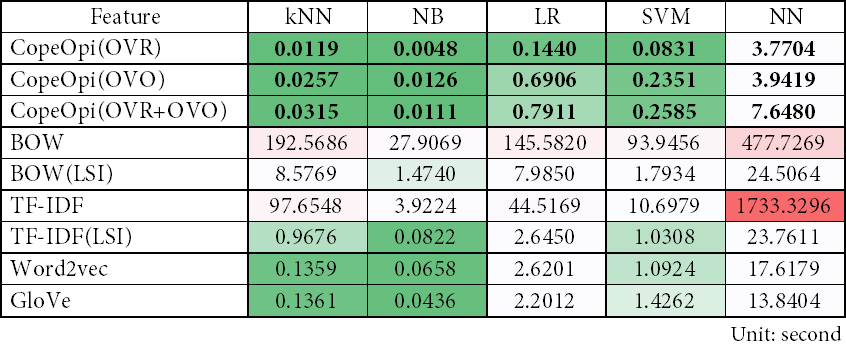
\includegraphics[width=\resultfigwidth]{chapters/ch4/table/tc/TC(ZH)(B)T.png}
\end{subtable}
\end{table}
\vspace{-1.75\intextsep}
\begin{table}[H]
\caption{Results of TC(ZH)(C)}
\label{tab:tc_zh_c}
\centering
\begin{subtable}{\textwidth}
	\centering
	\caption{Macro \fscore{}}
	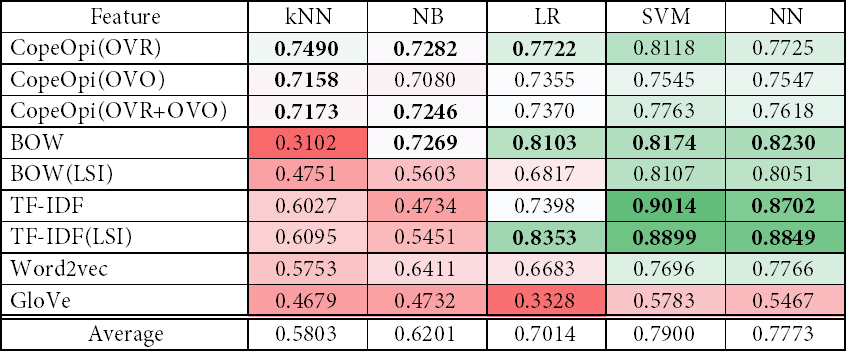
\includegraphics[width=\resultfigwidth]{chapters/ch4/table/tc/TC(ZH)(C).png}
\end{subtable}
\\[\tblskip]
\begin{subtable}{\textwidth}
	\centering
	\caption{Training CPU Time}
	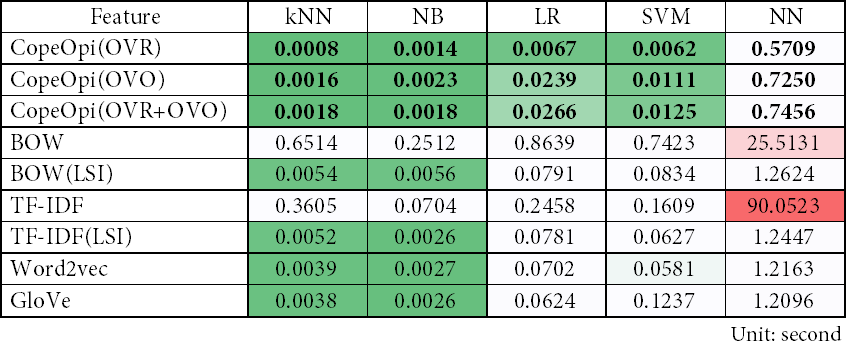
\includegraphics[width=\resultfigwidth]{chapters/ch4/table/tc/TC(ZH)(C)T.png}
\end{subtable}
\end{table}


\section{Summary}
Here we summarize our observations about CopeOpi vectors:
\begin{enumerate}
\item CopeOpi vectors can produce comparable results with a smaller vector size and shorter training time in multiclass text classification.
\begin{enumerate}[label=(\roman*)]
\item $\frac{49}{55}$ of the best macro \fscore{}s of CopeOpi vectors in multiclass classification are better than the average macro \fscore{} of each classifier of each experiment.
\item The vector size of CopeOpi vectors is the smallest in all experiment, as listed in Table~\ref{tab:vec_size}.
\item The training time of CopeOpi vectors is the shortest in all experiment.
\end{enumerate}
\item Compared with the other features, CopeOpi vectors provide stabler results when applied to different types of machine learning algorithms. There are some results deviating, but in those cases the deviations are general phenomenons for most of the features.
\item Compared with the winner TF-IDF, CopeOpi vectors lose by at most 3.02\% except the experiments without sufficient training instances. Although TF-IDFs perform the best, they also costs most in terms of memory space and training time. Since the vector size of TF-IDFs is proportional to the number of unique words in a corpus, in the cases of large corpus, CopeOpi vectors will have advantages in efficiency.
\end{enumerate}
\begin{table}[h]
\footnotesize
\centering
\caption{The vector sizes in experiments}
\label{tab:vec_size}
\scalebox{0.8}{
\begin{tabular}{|l|c|c|c|c|c|c|c|c|c|c|c|c|c|}
\hline
\multirow{3}{*}{} & \multicolumn{6}{c|}{SA}                                             & \multicolumn{7}{c|}{TC}                                \\ \cline{2-14} 
                  & \multicolumn{3}{c|}{(EN)}        & \multicolumn{3}{c|}{(ZH)}        & \multicolumn{4}{c|}{(EN)}  & \multicolumn{3}{c|}{(ZH)} \\ \cline{2-14} 
                  & (A)                & (B)  & (C)  & (A)                & (B)  & (C)  & (A)  & (B)  & (C)  & (D)   & (A)     & (B)    & (C)    \\ \hline
CopeOpi(OVR)      & \multirow{3}{*}{1} & 3    & 5    & \multirow{3}{*}{1} & 3    & 5    & 20   & 7    & 5    & 4     & 20      & 9      & 11     \\ \cline{1-1} \cline{3-4} \cline{6-14} 
CopeOpi(OVO)      &                    & 3    & 10   &                    & 3    & 10   & 190  & 21   & 10   & 6     & 190     & 36     & 55     \\ \cline{1-1} \cline{3-4} \cline{6-14} 
CopeOpi(OVR+OVO)  &                    & 6    & 15   &                    & 6    & 15   & 210  & 28   & 15   & 10    & 210     & 45     & 66     \\ \hline
BOW               & 3746               & 3846 & 3942 & 3108               & 3145 & 3148 & 8647 & 8647 & 8284 & 11851 & 46409   & 45992  & 23920  \\ \hline
BOW(LSA)          & \multicolumn{13}{c|}{200}                                                                                                    \\ \hline
TF-TDF            & 3746               & 3846 & 3942 & 3108               & 3145 & 3148 & 8647 & 8647 & 8284 & 11851 & 46409   & 45992  & 23920  \\ \hline
TF-TDF(LSA)       & \multicolumn{13}{c|}{200}                                                                                                    \\ \hline
Word2vec          & \multicolumn{13}{c|}{200}                                                                                                    \\ \hline
GloVe             & \multicolumn{13}{c|}{200}                                                                                                    \\ \hline
\end{tabular}}
\end{table}